\documentclass[%
	%draft,
	%submission,
	%compressed,
	final, %technote,
	%internal,
	%submitted,
	%inpress,
	%reprint,
	% %titlepage,
	notitlepage,
	%anonymous,
	narroweqnarray,
	inline,
	twoside,
        %invited,
	]{ieee}

\usepackage[top=3cm, bottom=2cm, left=1.5cm, right=1.5cm,a4paper,includeheadfoot]{geometry}



\usepackage[utf8]{inputenc}			% idioma
\usepackage[spanish]{babel}
\usepackage{float}
%\usepackage{color}
%\usepackage{colortbl}
%\usepackage{amsmath}
%\usepackage{amsfonts}
%\usepackage{verbatim}

\usepackage{hyperref}				% urls

% -------- PARA FIGURAS
\usepackage{graphicx}
%\usepackage{capt-of}
% -------- FIN FIGURAS

% -------- PARA MONXTRAR EL CODIGO DE MANERA AMENA
\usepackage{courier}
\usepackage{listings}
\lstset{ %
	language=C++,                % choose the language of the code
	basicstyle=\footnotesize\ttfamily,       % the size of the fonts that are used for the code
	numbersep=5pt,                  % how far the line-numbers are from the code
%	backgroundcolor=\color{white},  % choose the background color. You must add \usepackage{color}
	showspaces=false,               % show spaces adding particular underscores
	showstringspaces=false,         % underline spaces within strings
	showtabs=false,                 % show tabs within strings adding particular underscores
	frame=single,           % adds a frame around the code
	tabsize=6,          % sets default tabsize to 2 spaces
	captionpos=b,           % sets the caption-position to bottom
	breaklines=true,        % sets automatic line breaking
	breakatwhitespace=false,    % sets if automatic breaks should only happen at whitespace
}
% -------- FIN CODIGO

\hypersetup{			%sacar los colores horrendos de las ref
	colorlinks=false,
	pdfborder={0 0 0},
}


\begin{document}


\title[Wiretapping de paquetes ARP]{%
	Wiretapping de paquetes ARP: analizando redes locales usando Teor\'ia de la Informaci\'on
}

\author[CIRUELOS, MADDONNI, PATAN\'E]{
Gonzalo Ciruelos \authorinfo{G. Ciruelos e-mail: gonzalo.ciruelos@gmail.com},
\and{}Axel Maddonni\authorinfo{A. Maddonni, e-mail: axel.maddonni@gmail.com}%
\and{}y Federico Patan\'e\authorinfo{F. Patan\'e, e-mail: fedepatane20@gmail.com}
}

\journal{Grupo 13: Teor\'ia de las Comunicaciones, Departamento de Computaci\'on, UBA}

\firstpage{1}

\maketitle               


\begin{abstract} 
Con el objetivo de comprender diversos aspectos de una red local, nos planeteamos analizar sus paquetes ARP usando herramientas de la teor\'ia de la informaci\'on.
Para lograr eso, modelamos alg\'un aspecto de nuestra red como una fuente de informaci\'on, de manera de poder analizarla con las herramientas previamente dichas.
Adem\'as, comparamos distintos tipos de redes para poder confirmar o refutar nuestras hip\'otesis generales.
\end{abstract}

\begin{keywords}
ARP, LAN, broadcast, unicast, entrop\'ia, informaci\'on, Ethernet, Wi-Fi
\end{keywords}


\section{Introducci\'on te\'orica}

\PARstart En este trabajo nos proponemos utilizar herramientas de la Teor\'ia de la Informaci\'on y los paquetes ARP para intentar comprender diferentes redes locales. La pregunta que nos intentaremos responder en este trabajo es ?`Podemos conocer la topolog\'ia de la red y/o sus nodos m\'as importantes?

La explicaci\'on de las fuentes utilizadas vendr\'a m\'as adelante, pero es pertinente presentar el formato de los paquetes ARP. El protocolo de resoluci\'on de direcciones (Address Resolution Protocol) \cite{arp} es un protocolo usado para la resoluci\'on de direcciones de la capa de red a direcciones de la capa de enlace (usualmente MAC), lo que es una funci\'on cr\'itica en redes de m\'ultiple acceso.

Un paquete ARP tiene muchas partes, pero la que m\'as nos interesa es el campo OPER, o sea el campo de Operaci\'on, que nos indica qu\'e funci\'on cumple ese paquete. 
Los distintos valores de OPER en paquete ARP son is-at y who-has. 
Un paquete who-has es un paquete broadcast en el que una computadora pregunta al resto de la red qui\'en es la que tiene una direcci\'on de capa de red (generalmente IP) dada.
La respuesta a ese paquete es un paquete is-at, que es un paquete unicast, enviado desde la computadora con la direcci\'on de capa de red requerida hasta la computadora que emiti\'o el who-has.

Por otro lado, con respecto a la teor\'ia de la informaci\'on, utilizaremos los conceptos de informaci\'on y entrop\'ia cl\'asicos.


\section{Desarrollo}

\PARstart Como explicamos anteriormente, el trabajo se basará en analizar redes locales capturando paquetes ARP de redes locales y analizandolos utilizando herramientas de la teoría de la información.

Para capturar los paquetes de la red analizada, utilizamos el programa \textsc{Wireshark}. Luego, para postprocesar los datos y computar la inforamación pedida utilizamos la librería de Python \textsc{Scapy}. \textsc{Scapy} es una poderosa herramienta que permite capturar, decodificar, crear y envíar paquetes de manera muy sencilla.

\subsection{Ejercicio 1}

El ejercicio 1 proponía analizar los resultados modelando a los paquetes como una fuente de información muy simple: simplemente distinguir entre paquetes broadcast y paquetes unicast. La fuente consiste en dos símbolos, uno que representa a los paquetes unicast, y otro que representa a los paquetes broadcast.

Esta fuente no nos permitirá conocer muy bien quién es quién en la red, pero nos dará quizás un poco de información sobre lo que está pasando en la red local.

Que la cantidad de mensajes de broadcast sea muy grande, o sea, la información del símbolo que representa a los mensajes broadcast sea muy chica, será lo esperado. Esto se debe a que en una red normal, en la cual podemos escuchar todo lo que está pasando, lo esperable es que los dispositivos se comuniquen unos con otros en vez de estar envíando broadcasts todo el tiempo.

De alguna manera, si vemos pocos paquetes unicast, o sea que la información de este símbolo es muy alta, puede significar dos cosas:

\begin{enumerate}
  \item No tenemos visibilidad total de la red, por ejemplo porque está switcheada, y entonces vemos solo los paquetes unicast dirigidos a nuestro host.
  \item No hay comunicación efectiva entre los hosts de la red, porque los paquetes unicast de alguna manera miden cuanta comunicación de un host a otro está sucediendo.
\end{enumerate}

Nuestra implementación de este ejercicio puede verse en el archivo \texttt{ejercicio1.py}.


\subsection{Ejercicio 2}

El ejercicio 2 proponía que diseñemos una fuente de memoria nula en base a los paquetes ARP, que nos permitiera distinguir a los nodos distinguidos de la red, para alguna definición que demos de nodo distinguido.

Experimentamos con varias fuentes, y terminamos seleccionando que la fuente sea el destino de los paquetes who-has, por las siguientes razones:

\begin{enumerate}
  \item Si estamos analizando una red switcheada o muy subdividida en subredes virtuales (VLANs), entonces lo más probable es que solo recibamos paquetes who-has, dado que estos paquetes se envían en modo broadcast.
    Por esta razón los switches de la red local no los filtran y le llegan a todos los hosts.  Quizás esta diferencia no sea notable en redes inalámbricas, pero en redes cableadas complejas, que generalmente tienen switches, puede hacer una gran diferencia.
  \item Como justificamos anteriormente, vamos a usar paquetes who-has, ahora bien, la pregunta es porqu\'e el destino de esos paquetes. En este caso la respuesta es más obvia: si un host es el destinatario de más paquetes ARP, entonces es más requerido por el resto de los hosts, entonces es más probable que sea un nodo distinguido, como por ejemplo un router.
\end{enumerate}

Siguiendo estos simples preceptos, diseñamos nuestra fuente de información S1. Nuestra implementación de este ejercicio puede verse en el archivo \texttt{ejercicio2.py}.

\subsection{Grafo de la red}

Para los tres experimentos que realizamos, hicimos el grafo de la red que se desprende de los paquetes ARP enviados a lo largo de la captura.

El grafo fue realizado de la manera más natural. Por cada mensaje who-has capturado, el grafo tendrá una arista. Además, esa arista irá del nodo con IP igual a la IP fuente del who-has al nodo con IP destino del who-has.

Por razones de comodidad, solo mostramos aquellos nodos relevantes, es decir, los que tienen información baja con respecto a la fuente de información que S1.

Además, juntamos en uno a todos los hosts que tienen exactamente el mismo conjunto de aristas adyacentes. Esto se indicara con un [X]: si un nodo tiene [X] significa que ahí condensamos X cantidad de hosts, que tienen todos exactamente la misma conectividad que el nodo representado. 

Además, marcamos con un cuadrado aquellos nodos distinguidos según la fuente S1, es decir, aquellos que tienen menos información que la entropía.


\subsection{Conceptos generales}

\subsubsection{Gratuitous ARP}

En todos los experimentos apareció un tipo de paquete ARP llamado Gratuitous ARP, con lo cual nos parece mejor introducirlo al principio para dejar en claro qu\'e es y por qu\'e aparece en todos los experimentos.

Gratuitous ARP puede significar tanto un reply (is-at) como un request (who-has). Gratuito en este caso quiere decir que un request o un reply no es normalmente requerido de acuerdo con la especificacion de ARP (RFC 826) \cite{arp}, pero puede ser usado en algunos casos.
Un request ARP gratuito es un paquete donde la IP source y destination están ambas seteadas a la IP del host que envía el paquete. Además, la MAC destino es la dirección de broadcast \texttt{ff:ff:ff:ff:ff:ff}. Ordinariamente, no habrá respuesta para tal request.

Los ARP gratuitos tienen varias utilidades:

\begin{enumerate}
  \item Pueden ayudar a detectar conflictos de IP. Si un host recibe un paquete ARP que contiene una IP source que coincide con la suya, sabe que hay un conflicto.
  \item Ayuda a actualizar las tablas ARP de los hosts de la red.
  \item Cada vez que una interfaz IP se prende, el driver de la interfaz típicamente envía paquetes ARP gratuitos para precargar las tablas ARP de todos los hosts. Por eso, si un host envía muchos paquetes ARP gratuitos, podemos inferir que algo malo está sucediendo con \'el, por ejemplo que se está reiniciando o que su interfaz IP se reinicia continuamente porque no puede iniciarse correctamente.
\end{enumerate}


\subsubsection{Dirección 169.254.255.255}
[eg an address you end up picking yourself because DHCP didn't work usually picked using some arp to figure out if it belongs to someone else]


\section{Experimento 1}

El primer experimento que presentamos en el trabajo fue realizado en una cafetería (Starbucks), por la tarde, mientras había aproximadamente unas 15 personas a la vista usando dispositivos móviles. La captura de paquetes duró casi una hora.

\subsection{Resultados}

Primero, la fuente S. Nuestra hipótesis sobre esta fuente, basándonos en lo que dijimos anteriormente en el trabajo, es que el símbolo de los paquetes de broadcast tendrá una información mucho más alta que el símbolo de los paquetes unicast.

\begin{figure}[H]
  \centering
  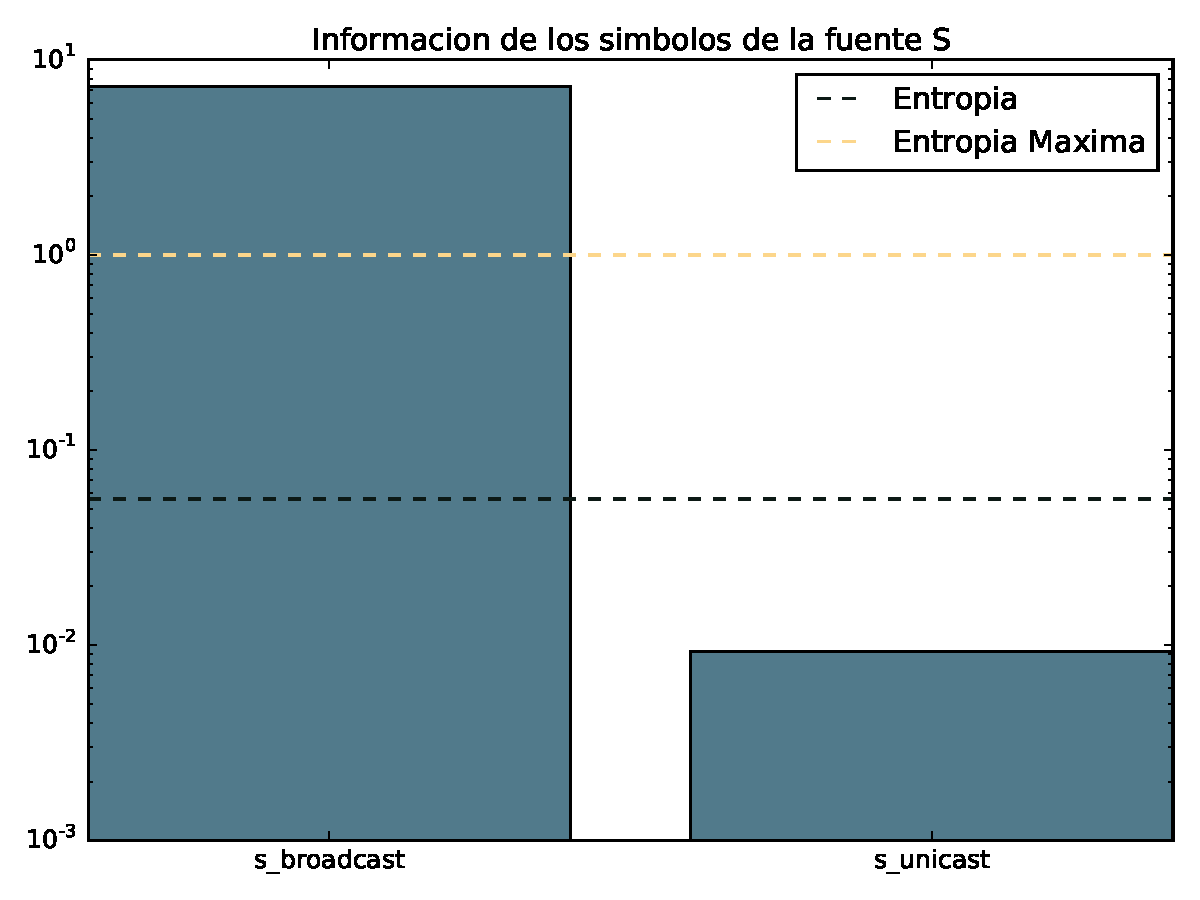
\includegraphics[width=8.5cm]{exp_starbucks/grafico1.pdf}
  \caption{\normalfont }
\end{figure}

Nuestra hipótesis sobre la red es que habrá unos pocos dispositivos que se conectarán a un router, y quizás si el router y el Access Point tengan ambos IPs dentro de la red, aparezcan como dispositivos separados en la misma.
Analizaremos esto, y todas nuestras otras hipótesis en la discusión.

\begin{figure}[H]
  \centering
  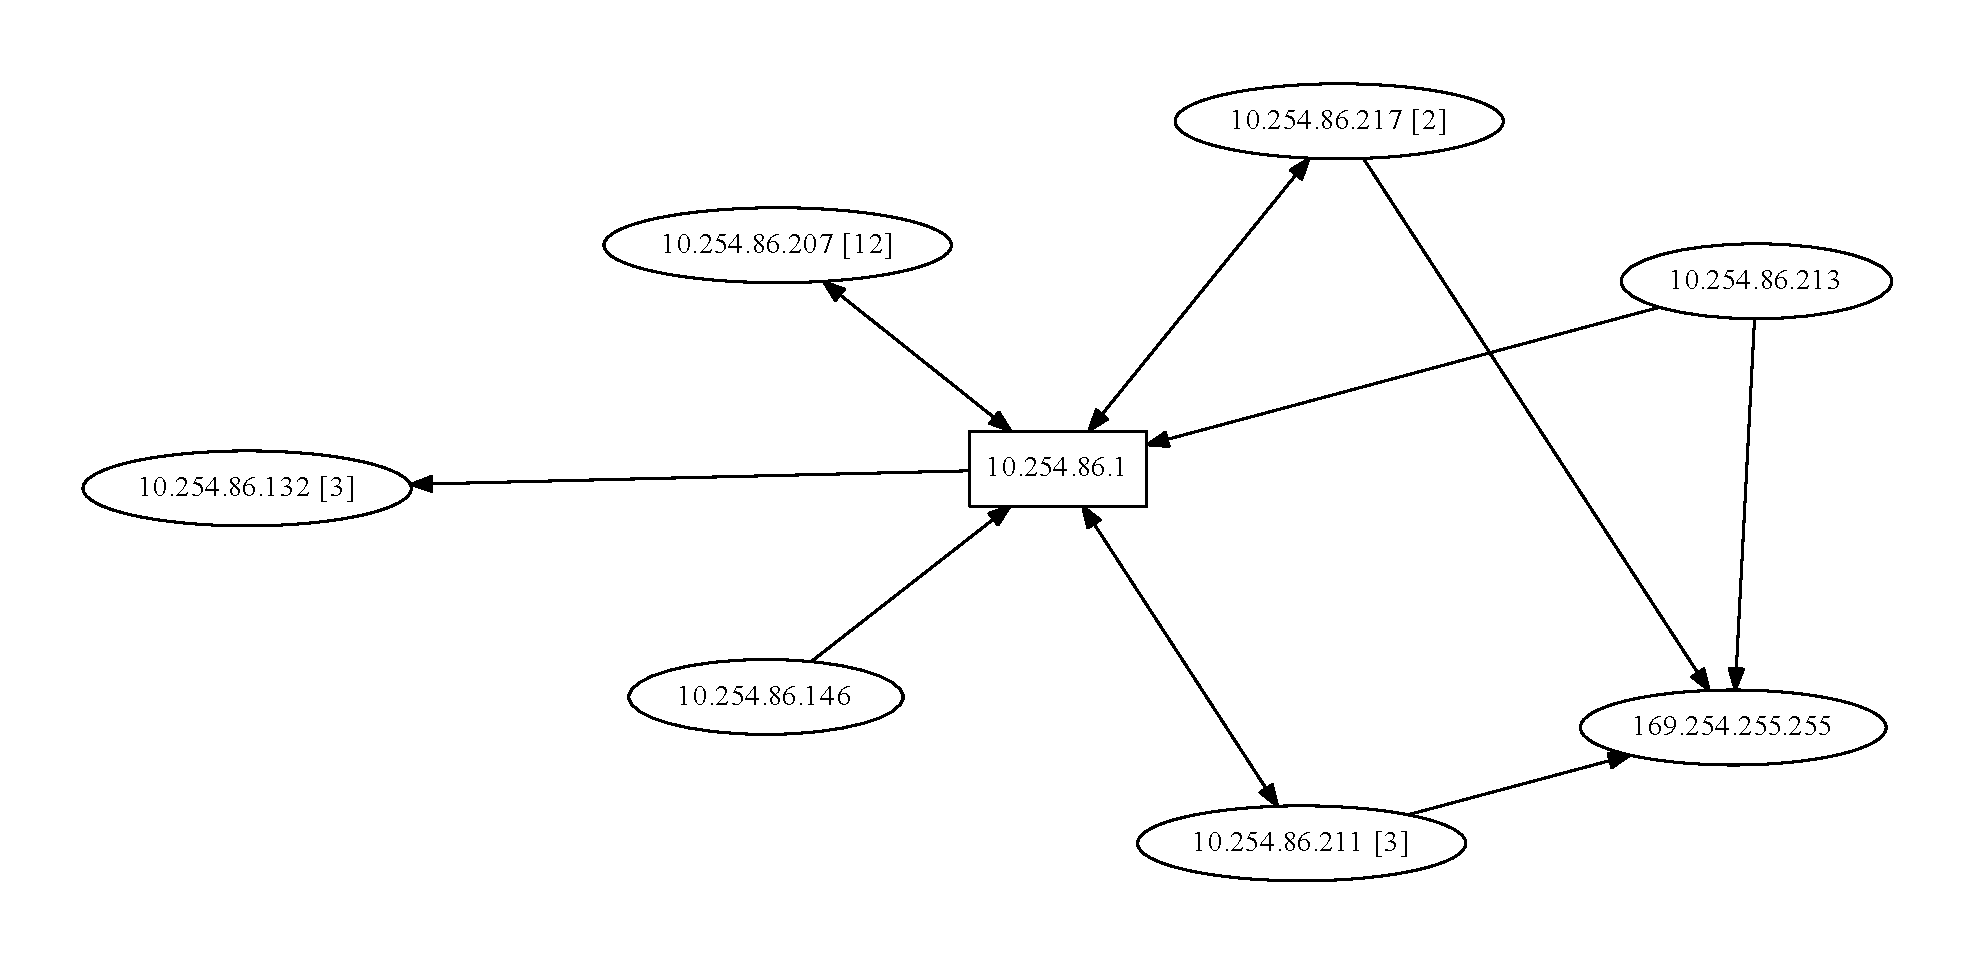
\includegraphics[width=8.5cm]{exp_starbucks/grafico2.pdf}
  \caption{  \normalfont Grafo de conectividad de la red, inferido de los paquetes who-has. Para ver con mayor detalle, se puede hacer zoom-in en el pdf. }
\end{figure}

Sobre la fuente S1, esperaremos que haya un dispositivo que tenga menor información que el resto, y esperaremos que este sea el router. Además, esperamos que el resto de los dispositivos sean hosts, y tengan menor información si son más activos en la red.

\begin{figure}[H]
  \centering
  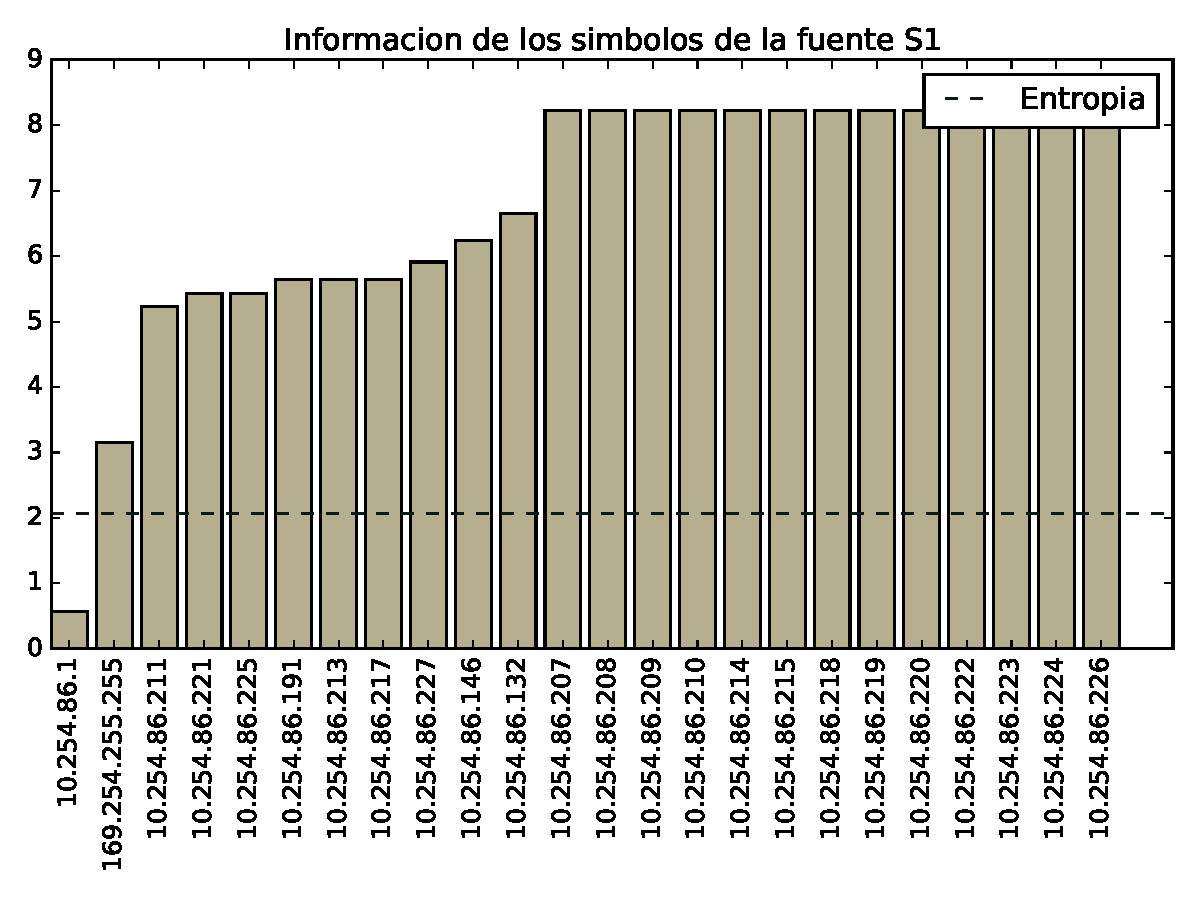
\includegraphics[width=8.5cm]{exp_starbucks/grafico3.pdf}
  \caption{ \normalfont Información de los símbolos de la fuente S1: solamente los nodos con menor información son representados.}
\end{figure}

\subsection{Discusión}

Analicemos los resultados que vimos en la sección anterior.

Empecemos por la fuente S. Como esperábamos, la información del símbolo asociado a los paquetes broadcast es muy alta. Como dijimos al principio del trabajo, asociaremos esto a dos hechos: 

\begin{enumerate}
  \item Podemos ver todo lo que pasa en la red, en particular, podemos ver todos los paquetes que se le envían a los demás hosts.
    Esto en general nos va a permitir inferir o bien que la red es una red Wi-Fi, o bien que es una red Ethernet muy simple, sin switches o subnets.
  \item Además, que la comunicación en la red es efectiva, o sea que los hosts están comunicando cosas unos con otros o bien con dispositivos fuera de la red.
    Si la mayoría de los paquetes fuera broadcast, eso nos daría la idea de que no se está dando comunicación efectiva entre los hosts, si no, que por ejemplo, todos los mensajes que se intercambian son de control.
\end{enumerate}

Por esa razón, es mucho más común en este caso que un paquete sea unicast que broadcast. Por ello, la entropía de la fuente S no va a ser máxima, dado que la información de los únicos dos símbolos es muy diferente.

Continuando con el análisis del grafo de la red y la fuente S1, se observa que hay 24 nodos. El nodo distinguido (según la fuente S1) es lo que parece ser el router. Inferimos que es el router porque su último octeto es 1, que es el valor default para routers. 

Las IP de los nodos corresponde a la red 10.254.86.0/24. La mayoría de los hosts terminaban en octetos distintos de 1, excepto el router, que como dijimos tenía a 1 como último octeto. Esto nos da la pauta de que efectivamente lo que estamos viendo es una red, que además se corresponde con la red Wi-Fi de la cafetería.

Nos parece razonable afirmar que el resto de los nodos son hosts conectados a la red Wi-Fi, dado que por lo que se veía en la cafetería, había un mínimo de 15 dispositivos conectados a la red, y además el resto se comporta de la misma manera. 

Notemos que los nodos que no se conectan solamente con el router (10.254.86.1), se conectan con el nodo 169.254.255.255. El nodo que tiene esta IP es un caso que puede ser considerado anómalo o borde y fue explicado anteriormente. Es importante decir que apareció en todos los experimentos con Wi-Fi que hicimos, con lo cual es interesante tenerlo en cuenta para futuros experimentos.

La cantidad de nodos del grafo indica que los dispositivos conectados a la red Wi-Fi son los que observamos, más algunos que no pudimos ver.

Es muy interesante que la fuente propuesta y nuestro grafo de nodos nos permitió de una manera muy precisa comprender la disposición y organización de la red. En las conclusiones haremos un análisis general de este y el resto de los experimentos.








\section{Experimento 2}

El segundo experimento que mostraremos fue realizado en los laboratorios del Departamento de Computación de FCEyN, más especificamente en el laboratorio 2.
La captura de paquetes duró una hora y se realizó sobre la red cableada del laboratorio, es decir, sobre Ethernet.
La modalidad fue desenchufar el cable Ethernet de la computadora 3 del laboratorio 2, y enchufandolo en nuestra propia computadora, de tal manera de poder capturar paquetes en modo promiscuo.

La captura de paquetes se realizó durante la tarde, mientras había aproximadamente 10 personas utilizando las computadoras de ese laboratorio. Las mediciones fueron realizadas con la autorización de uno de los administradores de la red, quien además ayudó a verificar las teorías que extrajimos de los paquetes. Veremos todo esto más adelante.

Antes de pasar a ver los resultados, una cosa que vale la pena decir es que, por como es la red de los laboratorios, al haber utilizado una computadora distinta de la de los labos para realizar las mediciones, la red no nos asignó IP, es decir, no nos ``conectó'' de manera total a la red local. Sin embargo, esto no perjudicó en nada a las mediciones, y solo se vió reflejado en la fuente S.


\subsection{Resultados}

Primero analicemos la fuente S, que es la fuente de los paquetes unicast y broadcast. Como dijimos anteriormente, no teníamos dirección IP asignada. Esto sumado a que la red es switcheada, nos hace esperar que la cantidad de paquetes unicast que vamos a ver sea mucho más baja que lo normal. Esto, dicho en lenguaje de la Teoría de la Información, es que el símbolo que representa a los mensajes unicast tendrá una información más baja de la esperada.

Sin embargo, por como está configurada la red del laboratorio, sabemos que detrás de cada switch hay aproximadamente 4 o 5 computadoras, con lo cual podremos ver algunos paquetes unicast. Veamos qu\'e pasó.

\begin{figure}[H]
  \centering
  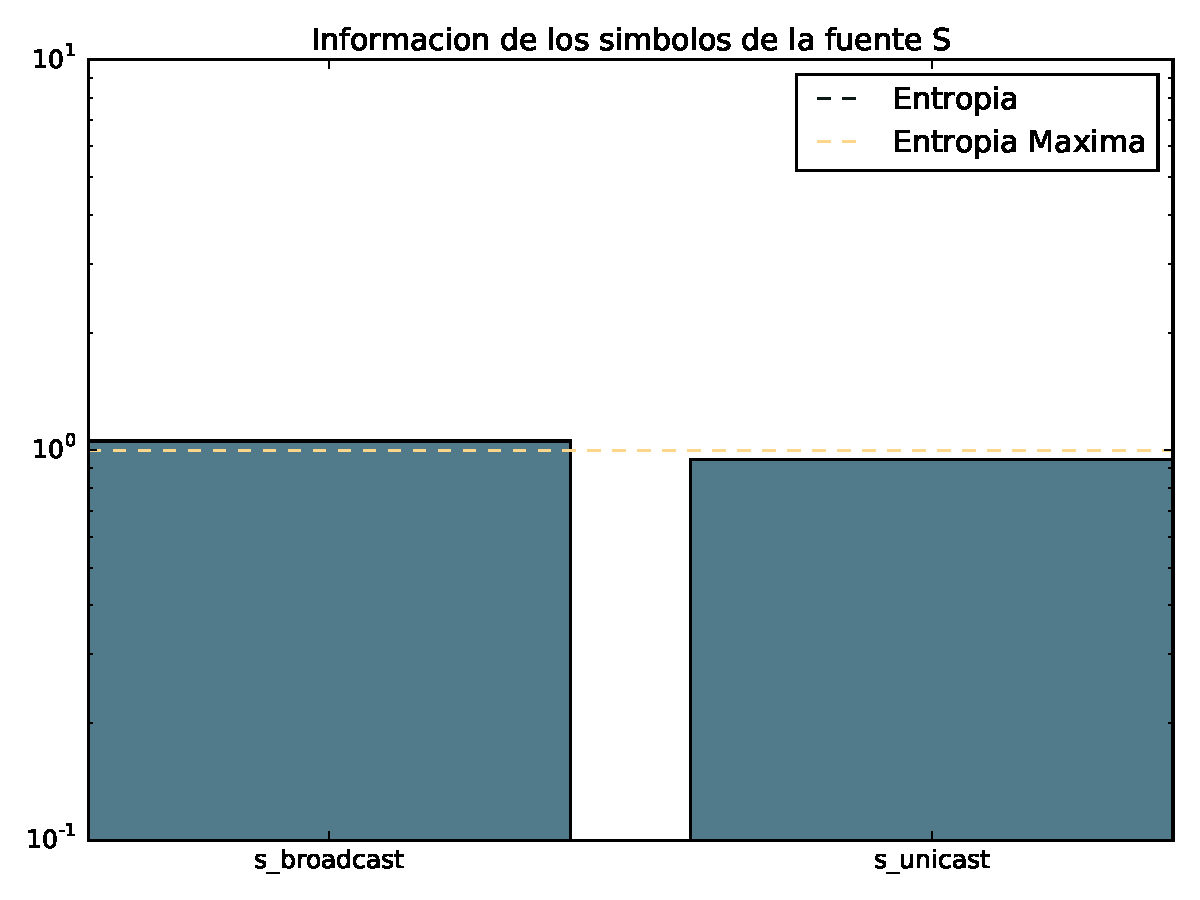
\includegraphics[width=8.5cm]{exp_labo/grafico1.pdf}
  \caption{\normalfont }
\end{figure}


Ahora pasemos a ver el diagrama de conectividad de la red, que nos permitirá saber más sobre cómo está configurada.

\begin{figure}[H]
  \centering
  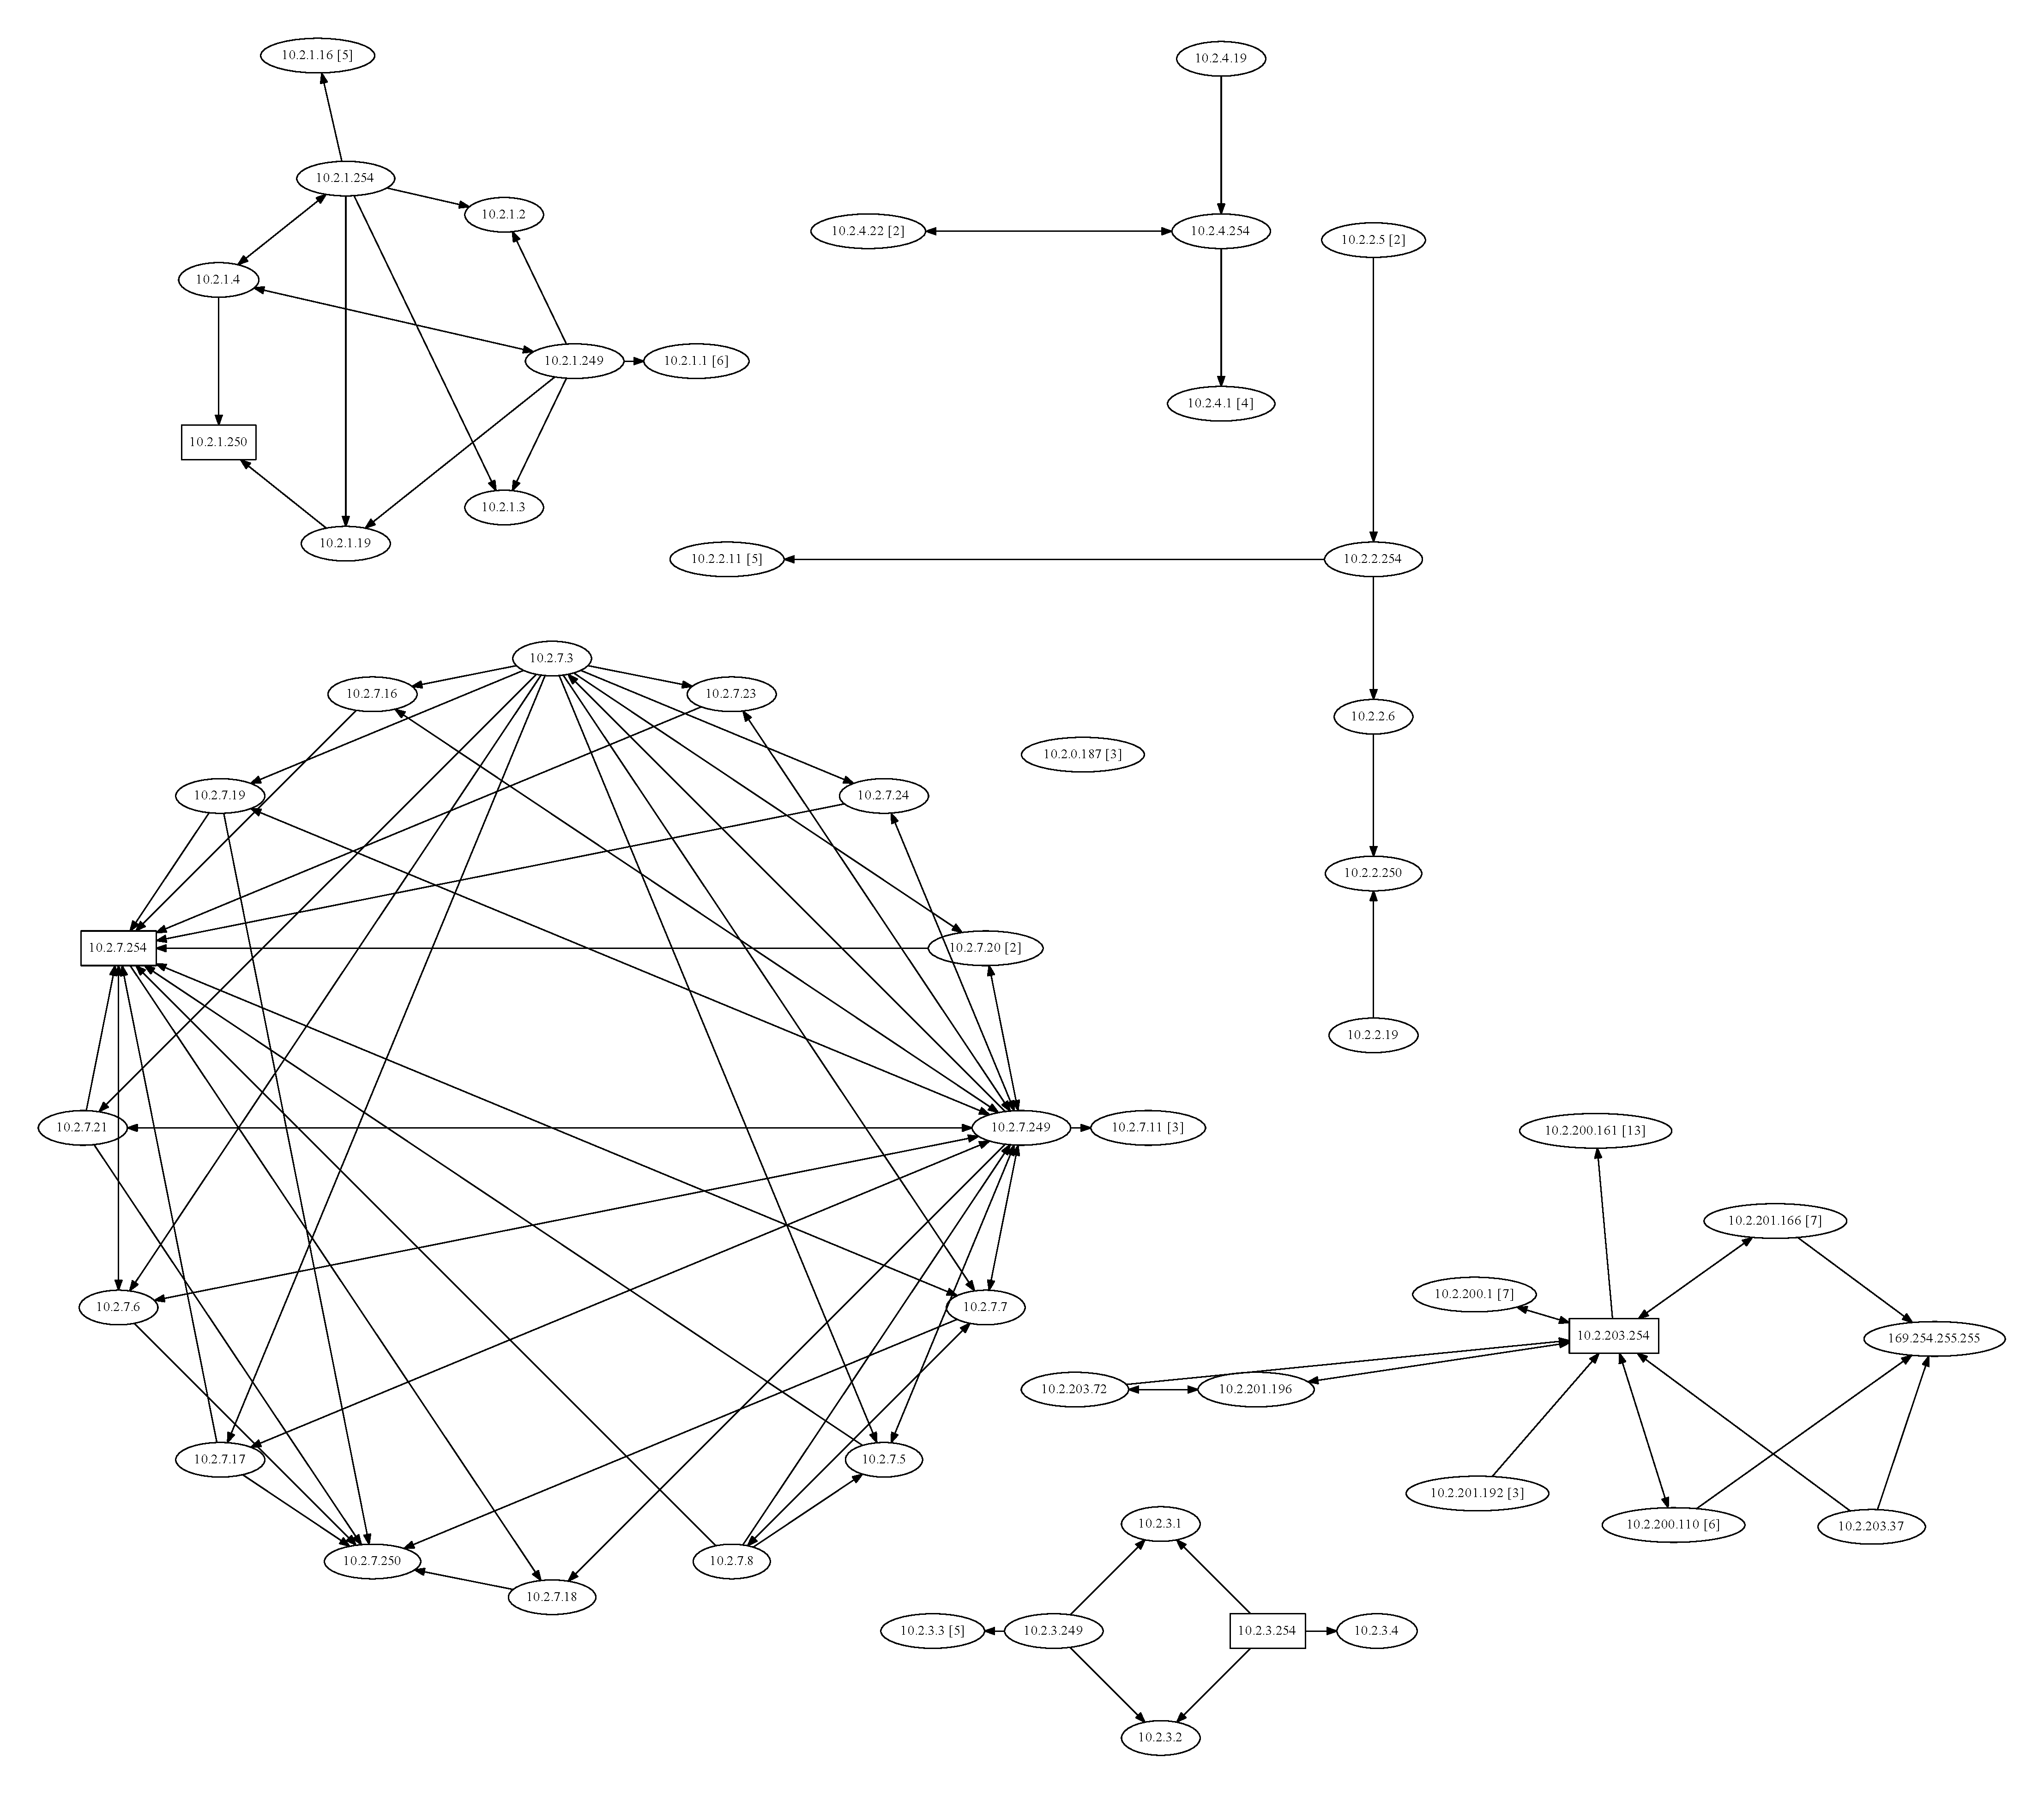
\includegraphics[width=8.5cm]{exp_labo/grafico2.pdf}
  \caption{  \normalfont Grafo de conectividad de la red, inferido de los paquetes who-has. Para ver con mayor detalle, se puede hacer zoom-in en el pdf. }
\end{figure}


\begin{figure}[H]
  \centering
  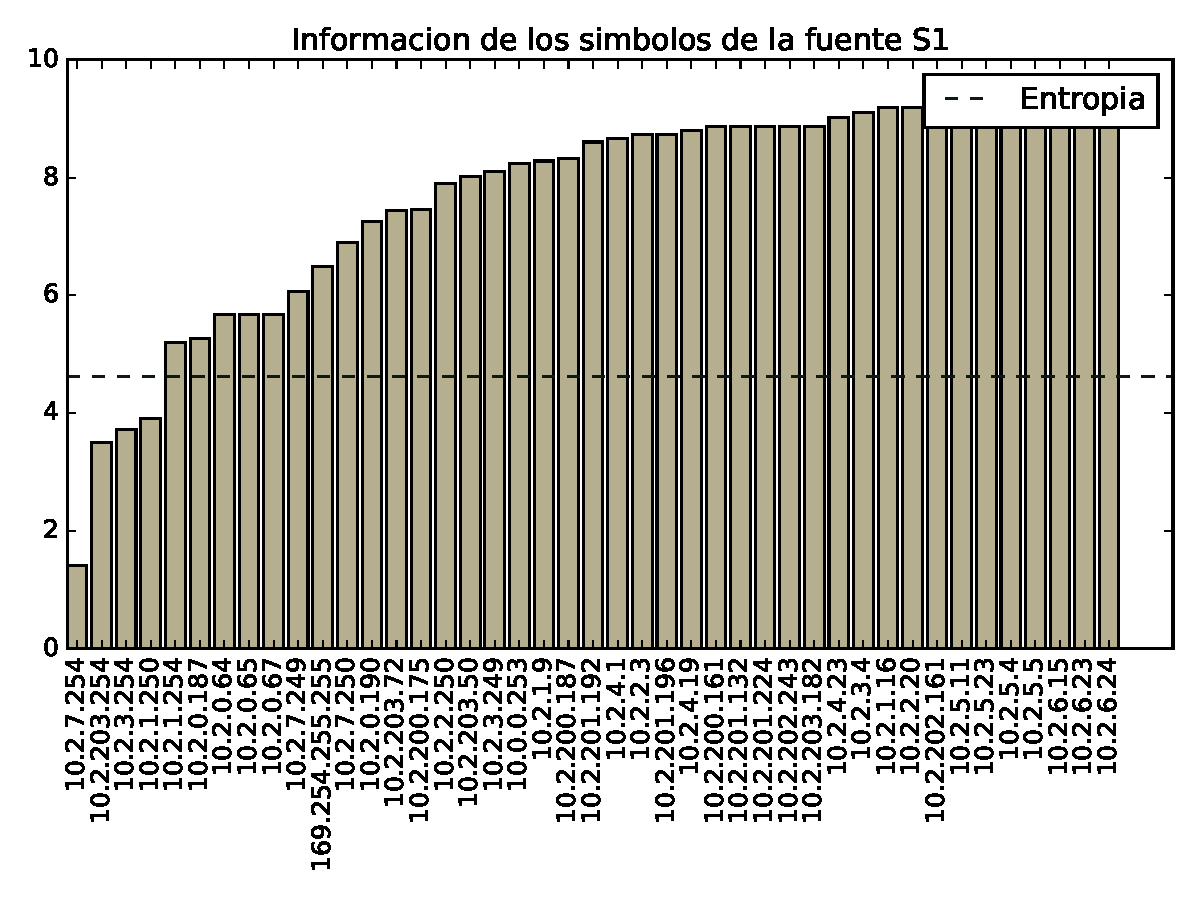
\includegraphics[width=8.5cm]{exp_labo/grafico3.pdf}
  \caption{ \normalfont Información de los símbolos de la fuente S1: solamente los nodos con menor información son representados.}
\end{figure}

\subsection{Discusión}

Para empezar, se confirma lo que dijimos sobre la fuente S: la información del símbolo de los paquetes unicast es mucho más alta de lo esperada e iguala casi a la de los paquetes broadcast. Esto provoca que la entropía sea muy cercana a la máxima. Desde el punto de vista de la probabilidad, esta fuente es menos predecible que la que vimos antes.

Además, si no hubieramos sabido como estaba la configurada la red (que se ve a simple vista en los laboratorios), podríamos haber inferido que está fuertemente switcheada dada la información de estos símbolos.

Con lo cual, como dijimos al principio del trabajo, esta fuente nos permite saber, entre otras cosas, que tanta visibilidad tenemos de toda la red: a más visibilidad más paquetes unicast nos van a llegar, por lo tanto más baja va a ser la información del símbolo asociado.



Para continuar con el grafo de conectividad y la fuente S1, como vemos, hay muchos dispositivos en la red, contamos más de 100 dispositivos. Sin embargo, solo mostramos aquellos relevantes para la discusión. Esta cantidad nos dice que la red es muy compleja, y que salvo excepciones, seguramente tendrá alguna subestructuración interna, por ejemplo subnetting, y que por lo tanto será un desafío intentar comprenderla.


Yendo más a lo específico, se ve que hay un grafo muy similar a un grafo completo, que tiene un nodo distinguido con IP 10.2.7.254. Nuestra hipótesis será que este dispositivo es el router.
Además, todos los nodos de ese subgrafo tienen IPs de la forma 10.2.7.XXX.
Es decir, ese subgrafo representa la subred 10.2.7.0/24.
Por la cantidad y el detalle de nodos observados en esta subred, podemos inferir que es la red del laboratorio 2, donde capturamos los paquetes.
Sin embargo de ninguna manera podemos imaginarnos por que tantas de las computadoras se envían paquetes ARP unas a otras. Veremos la razón de esto más adelante.

Además, podemos observar que se repite el mismo patrón en distintos lugares, por lo que podemos asumir que son los distintos laboratorios. El patrón al que nos referimos es la IP de la pinta 10.2.n.XXX, donde n es el número de laboratorio y XXX es el número de host. Además, como antes, 10.2.n.254 suele ser el nodo distinguido, con lo cual podemos asumir que todos esos son los routers de cada labo.

Hay otras 2 partes de la red que nos gustaría analizar. Primero, tres nodos de IP 10.2.0.XX, que lo único que hacen es mandar Gratitious ARP. Como vimos anteriormente, un Gratuitious ARP son paquetes broadcast que actúan como paquetes is-at, pero que nunca fueron pedidos.
Estos dispositivos actúan de manera anómala, pero como la red es muy compleja, podemos establecer como hipótesis que son dispositivos de control de la red.

Por último, podemos analizar la subred que se encuentra en la parte inferior izquierda de la figura. Como puede apreciarse, es bastante distinta al resto de las redes. 

Esta red sigue un patrón muy similar al que observamos anteriormente en la red Wi-Fi. Además, aparece la misma IP que había aparecido antes: 169.254.255.255. Por último, esta subred tiene un nodo distinguido terminado en 254: 10.2.203.254, así que nuestra hipótesis será que esta subred representa parte de la red Wi-Fi de los laboratorios de la facultad.


Luego de plantear todas nuestras hipótesis, nos pareció interesante consultar con un administrador de la red para saber que tan exactas fueron nuestras predicciones utilizando un modelo tan simple como usamos.

Resultó que nuestras predicciones fueron muy acertadas. Como predijimos, cada labo se representa internamente con una subred. Estas subredes son las de la pinta 10.2.n.0/24. Además, los routers de cada labo son los de IP 10.2.n.254, como habíamos predicho.

Finalmente, el subgrafo que creíamos que se correspondía con la red Wi-Fi, efectivamente lo hacía. Según el administrador, esa subred corresponde a IPs de un pool dinámico de IPs, que se asignan en el rango de direcciones de 10.2.200.0 a 10.2.201.255 de forma dinámica cada vez que un dispositivo nuevo se conecta a la red. ado que el Wi-Fi de los laboratorios está configurado con un pool dinamico de direcciones, y 10.2.203.254 es el router de la red. Quizás era un poco dificil
conocer toda esta información solamente con el grafo de conexiones, pero nos parece muy interesante contarlo de todas formas, porque es un patrón recurrente en redes Wi-Fi.

Además, nos aclaró que el hecho que las PCs de los laboratorios se manden paquetes unas a otras es esperado y tiene variadas causas. Primero, puede ser que dos usuarios esten usando un programa que use la red local, y entonces las computadoras se van a enviar paquetes ARP entre ellas. 
Otra cosa que sucede, es que las redes de los laboratorios tienen software de control y mantenimiento por temas de seguridad, y sobre todo para hacer que la red sea más fácil de mantener. Además es algo necesario para poder implementar el sistema conocido como Milagro, para poder conectarse a los labos a trav\'es de ssh.

Por último, el administrador desconocía la razón por la cual había ciertos nodos que lo único que hacían era enviar Gratuitous ARP. Nos parece interesante plantear este interrogante como trabajo futuro.


\section{Experimento 3}

\PARstart El último experimento presentado fue realizado en una oficina con aproximadamente 20 empleados trabajando, en horario laboral. La captura de paquetes se realizó sobre la red Wi-Fi de la empresa a la que se conectan la mayoría de los dispositivos móviles y notebooks.

\subsection{Resultados}

Para la primera fuente,  esperaremos que la información del símbolo que representa a los paquetes broadcast sea mayor, debido a que la comunicación entre dispositivos tiende a ser unicast y no broadcast por lo que la cantidad de unicast es mayor.

\begin{figure}[H]
  \centering
  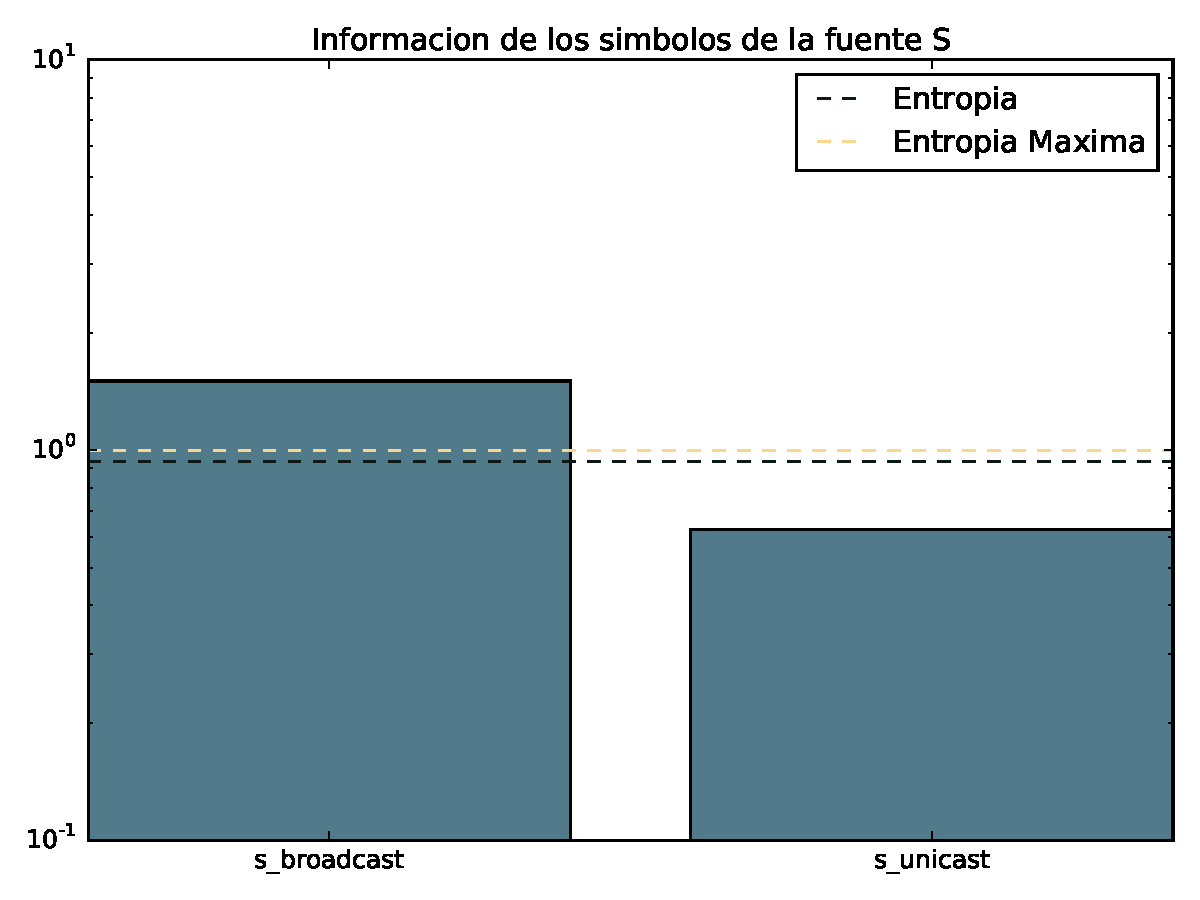
\includegraphics[width=8.5cm]{exp_empresa/grafico1.pdf}
  \caption{\normalfont }
\end{figure}

Esta red, al igual que la red analizada en el primer experimento corresponde a una red inalámbrica, por lo que se debería comportar de una manera similar a la del primer experimento, pero con una mayor cantidad de dispositivos de tipo host.

\begin{figure}[H]
  \centering
  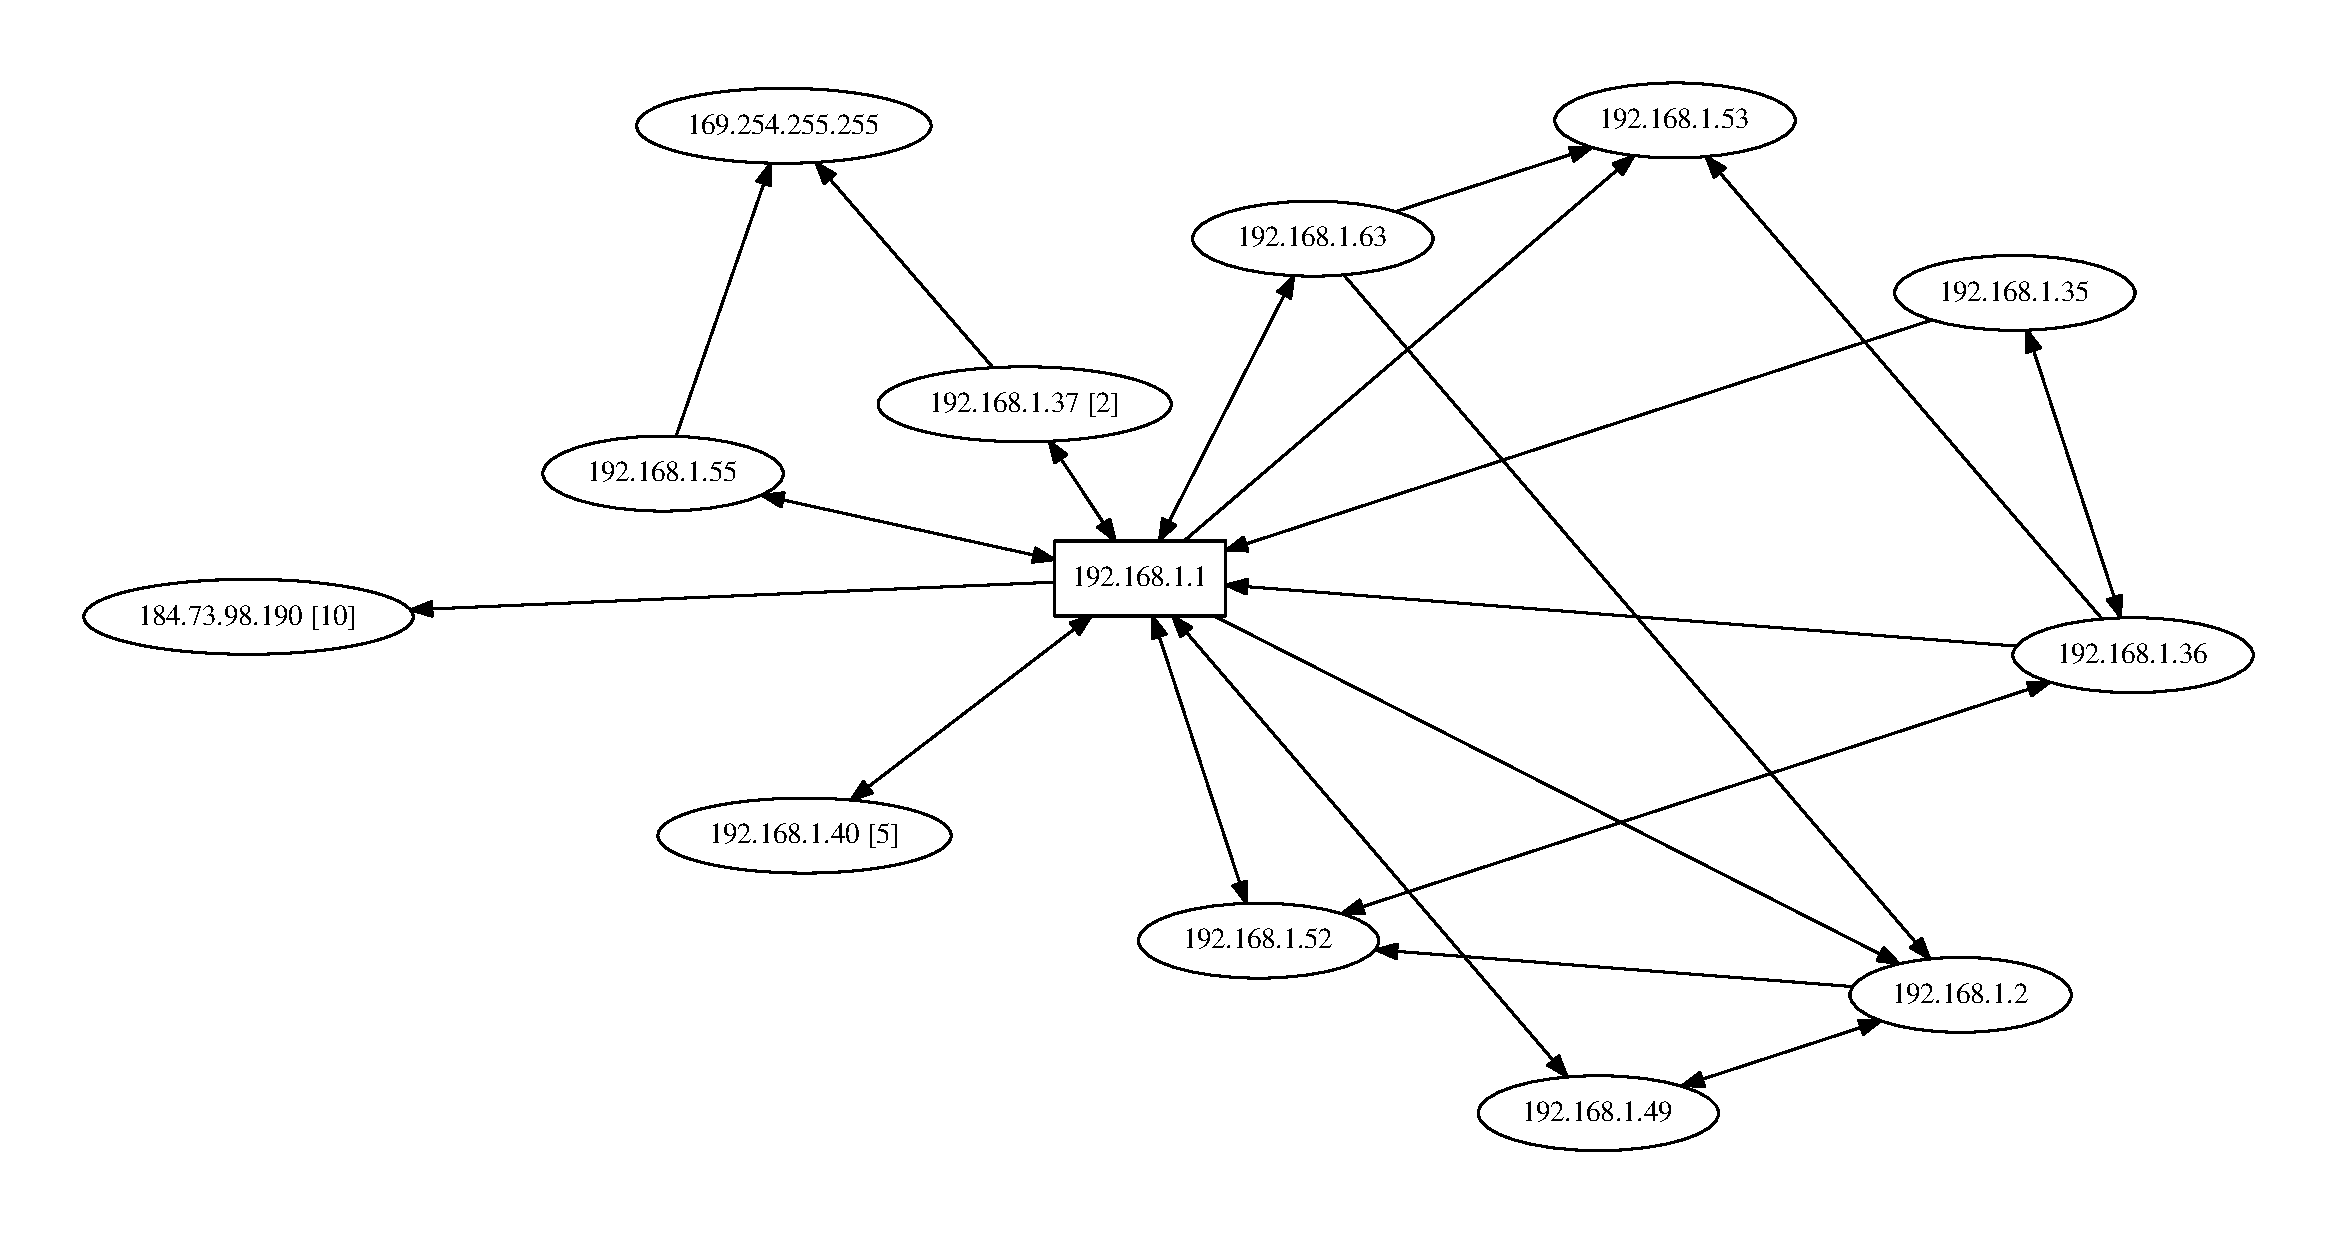
\includegraphics[width=8.5cm]{exp_empresa/grafico2.pdf}
  \caption{  \normalfont Grafo de conectividad de la red, inferido de los paquetes who-has. Para ver con mayor detalle, se puede hacer zoom-in en el pdf. }
\end{figure}

Esperaremos que a partir de la fuente S1 se destaque algún dispositivo que corresponderá al Default Gateway configurado en la tabla de routeo de los host (el router de la red).

\begin{figure}[H]
  \centering
  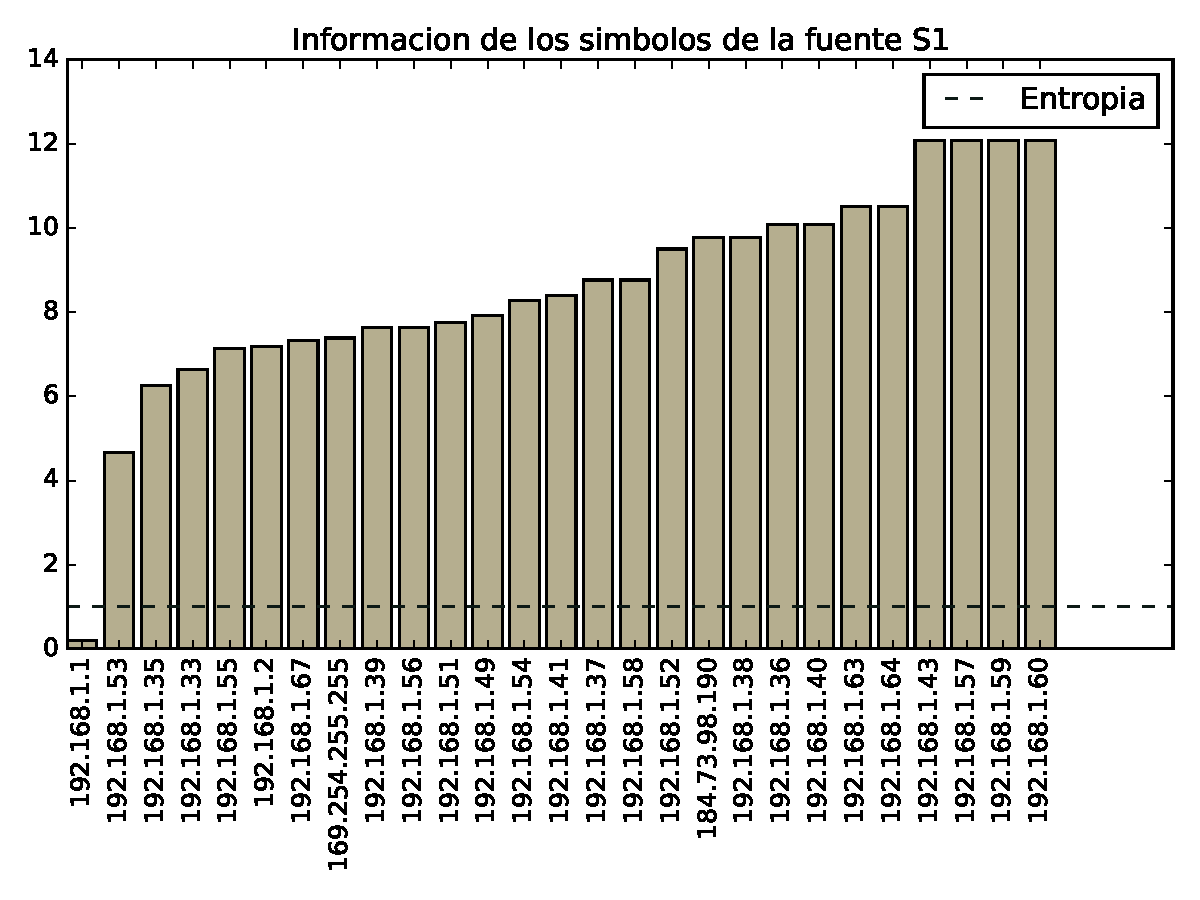
\includegraphics[width=8.5cm]{exp_empresa/grafico3.pdf}
  \caption{ \normalfont Información de los símbolos de la fuente S1: solamente los nodos con menor información son representados.}
\end{figure}

\subsection{Discusión}

Analicemos los resultados que vimos en la sección anterior.

En el gráfico correspondiente a la información de cada símbolo de la primera fuente, se puede observar, como predecíamos, que la información de los mensajes tipo broadcast es mayor. Sin embargo, a diferencia de la red Wi-Fi analizada en el primer experimento, la diferencia en este caso en menor debido a que la duración de la escucha en este experimento fue menor.

Como se ve en el gráfico, la entropía de la fuente está muy cercana a la entropía máximo debido a que la diferencia entre la información aportada por cada símbolo no es tan alta.

En el gráfico de topología de la red se puede observar al menos 15 direcciones de IP correspondientes a una misma red: 192.168.1.0 con una máscara de red 255.255.255.0 ya que todos los dispositivos tienen como último octeto valores entre 1 y 254. 

El dispositivo distinguido tiene como IP 192.168.1.1, que es la dirección usada normalmente para el router de la red, que se corresponde con el Default Gateway configurado en los hosts.

En el grafo de la red se puede ver claramente como todos los dispositivos de la red local se comunican con el que consideramos es el router, para acceder quizás a algún servidor externo, representado en el nodo con la IP 184.73.98.190. Notar que este nodo tiene un [10] debido a que hay 10 nodos con las mismas aristas, es decir que aparecen como destino de algún paquete enviado por el router, y no pertenecen a la red local.

Además, se puede notar que los hosts de la red local se comunican entre sí, fenómeno que no se observa en la red de Starbucks. Esto se debe a que en una red de tipo empresarial, los dispositivos locales tienden a comunicarse entre sí, por lo que se envían paquetes ARP preguntando por las IPs de los otros hosts de la red.

Por último, se puede observar la aparición del nodo 169.254.255.255, que como se mencionó anteriormente, corresponde a una dirección por default que se asignan los dispositivos debido a que DHCP no funcionó correctamente al asignar la IP.





\section{Conclusión}

Para concluir, podemos decir que nuestros experimentos fueron exitosos, dado que nos permitieron detallar y especificar técnicas para endender redes locales a partir de la escucha de paquetes ARP, lo que era el objetivo del trabajo.

Para resumir algunos puntos que fuimos dando a lo largo del trabajo para tener en cuenta al analizar redes usando esta técnica podemos decir:

\begin{enumerate}
  \item Si la fuente S tiene una entropía muy alta, quiere decir que la información del símbolo de los paquetes broadcast es muy similar a la información de los paquetes unicast. Esto significará en general que no tenemos visibilidad total de la red, o que el overhead de los paquetes de control es mucho, y no hay comunicación efectiva entre los hosts.
  \item En general los nodos con información menor con respecto a la fuente S1 son los routers o Default Gateways de la red.
  \item Las redes Wi-Fi son bastante simples y se asemejan a un grafo estrella, si no se tiene en cuenta la IP excepcional 169.254.255.255 que fue explicada en detalle anteriormente.
\end{enumerate}

Si queremos comparar las redes Wi-Fi y la redes ethernet, podemos decir que las primeras (en general) son más fáciles de analizar dado que la visibilidad que tenemos de los paquetes de la red es total, y por ejemplo la fuente S se va a comportar de la forma que esperamos.

Por otro lado, las redes Ethernet, si estan fuertemente switcheadas o subneteadas nos van a dar más sesgadas para el lado de los paquetes broadcast, dato que también podemos obtener de la fuente S1.

Fuera de eso, la diferencia no es muy grande. Es importante notar que fue vital nuestra eleccion de fuente S1 en este caso, dado que si hubiéramos elegido como fuente los paqutes is-at (unicast), la fuente hubiera dado muy mal para los casos Ethernet.


En cuanto al tamaño de las redes, la diferencia en la fuente S es casi nula. Sin embargo, en la fuente S1 se observa que la diferencia de información entre los nodos distinguidos y los nodos no distinguidos tiende a ser mayor en las redes más grandes.

La explicación de este fenómeno es realmente simple. A más nodos tiene una red, más nodos van a estar accediendo al router (o al nodo distinguido, sea lo que sea), con lo que va a haber muchos request ARP (who-has) a ese nodo, con lo que la información va a ser muy pequeña. Por otro lado, en redes más pequeñas, la información de los nodos distinguidos también va a ser pequeña, pero menos, dado que la cantidad de requests ARP que recibe va a ser menor en proporción.


Comparar la información de los símbolos de la fuente S1 con la entropía de la fuente S1 fue vital para encontrar los nodos distinguidos. Esto, como explicamos en la introducción, se justifica teóricamente dado que los nodos distinguidos van a ser más comunes como símbolos de la fuente S1 que el resto, con lo cual su información va a ser menor. En particular, un muy buen umbral que se puede elegir para decidir si un símbolo tiene menor información de la esperada es la entropía, dado
que la entropía es literalmente la esperanza de la información.

Una cosa importante para resaltar es que esperaremos que a más nodos haya en nuestra red, más grande sea la entropía. Esto se debe a que si hay muchos hosts en la red, esperamos que sean hosts comunes tipo PC, que en general reciben pocas requests ARP, con lo cual la información de su símbolo asociado va a ser muy alta, provocando que la esperanza de la información (es decir, la entropía), aumente. Por lo tanto, yendo hacia el lado contrario del argumento de recién, esperamos que
si la entropía es alta, entonces la cantidad de nodos no distinguidos sea mayor.
Esto es importante tenerlo en cuenta porque es un dato muy importante que podemos obtener de la red con solo saber la entropía de la fuente S1.

Por último, en general observamos que cuanto más alta es la entropía más nodos distinguidos hay. Esto tiene dos explicaciones posibles, que se complementan una con la otra.
Primero, la explicación numérica: como para nosotros un nodo es distinguido si la información de su símbolo asociado es menor que la entropía, si la entropía es más grande entonces es más probable (por probabilidad) que un símbolo cualquiera tenga menor información que el valor de la entropía.
Segundo, por un tema funcional, si en una red hay muchos nodos, es probable que esa red tenga algún tipo de subestructura y no tenga un único router adentro, si no que tenga varios. Por esa razón, si la entropía es más grande, esperamos que haya más nodos en general, por lo tanto más routers, luego más nodos distinguidos.




%----------------------------------------------------------------------

\begin{thebibliography}{1}

%\bibitem{enunciado}
%C\'atedra de Teor\'ia de las Comunicaciones\\
%\newblock {\em Primer trabajo pr\'actico}\\
%\newblock Primer cuatrimestre $2013$

\bibitem{arp}
RFC 826 - Ethernet Address Resolution Protocol\\
\url{http://tools.ietf.org/html/rfc826}\\
\newblock C. Plummer $1982$

%\bibitem{conflicto}
%RFC 5227 - IPv4 Address Conflict Detection\\
%\url{http://tools.ietf.org/html/rfc3927}\\
%\newblock S. Cheshire $2008$

%\bibitem{link}
%RFC 3927 - Configuration of IPv4 Link-Local Addresses\\
%\url{http://tools.ietf.org/html/rfc3927}\\
%\newblock Cheshire, et al. $2005$

%\bibitem{patente}
%Method and apparatus for detecting a router that improperly responds to ARP requests\\
%\newblock US 7729292 B2\\
%\url{http://www.google.com/patents/US7729292}\\
%\newblock Stuart D. Cheshire y Joshua V. Graessley

\bibitem{scapy}
\url{http://www.secdev.org/projects/scapy}

%\bibitem{tcp}
%\url{http://www.tcpdump.org}

\end{thebibliography}


\end{document}

